\documentclass[12pt,letter]{article}
\usepackage{mathptmx} % added for time new roman font
\usepackage[left=1in,right=1in,top=1in,bottom=1in]{geometry}
\usepackage[latin1]{inputenc}
\usepackage{amsmath}

% defines all example enviorment
\usepackage[framemethod=tikz]{mdframed} % added for the box around examples
\newtheorem{ex}{Example}
\numberwithin{ex}{section} % allows for the use of example numbers that lign up with the section numbers
\newenvironment{example}{\begin{mdframed}[middlelinewidth=0.5mm]\begin{ex}\normalfont}{\end{ex}\end{mdframed}}

% defines all review enviorment
\usepackage[framemethod=tikz]{mdframed} % added for the box around examples
\newtheorem{re}{Review}
\numberwithin{re}{section} % allows for the use of example numbers that lign up with the section numbers
\newenvironment{review}{\begin{mdframed}[middlelinewidth=2mm,roundcorner=20pt]\begin{re}\normalfont}{\end{re}\end{mdframed}}

% defines the quotation enviorment 
\usepackage{xcolor}
\newcommand{\quotebox}[2]{\begin{center}\fcolorbox{white}{blue!15!gray!15}{\begin{minipage}{0.9\linewidth}\vspace{10pt}\center\begin{minipage}{0.8\linewidth}{\space\Huge``}{#1}{\Huge''}{\break\null\hfill} {\small #2}  \end{minipage}\medbreak\end{minipage}}\end{center}}

% defines the definition enviorment 
\newcommand{\definitionbox}[2]{\begin{center}\fcolorbox{white}{blue!15!gray!15}{\begin{minipage}{0.9\linewidth}\vspace{10pt}\center\begin{minipage}{0.8\linewidth} {{\textbf{Definition} - }{#1}: {#2}}\end{minipage}\medbreak\end{minipage}}\end{center}}

\usepackage{amsfonts}
\usepackage{amssymb}
\usepackage{graphicx}
\usepackage{float}
\usepackage{booktabs}
%\usepackage{parskip} % remove all the paragraph indents

\usepackage{setspace}
%\usepackage[colorlinks=true]{hyperref}
\usepackage{textcomp} 
\usepackage{multicol} 


%%%%%%%		define the symbols for positive directions		%%%%%%
\makeatletter													%%	
																%%					
\newcommand*\curveplus{% positive counterclockwise				%%
  \mathbin{\rotatebox[origin=c]{90}{$\m@th\curvearrowleft$}+}}	%%
																%%
\newcommand*\rightplus{% positive right							%%
  \mathpalette\@rightplus\relax}								%%
\newcommand*\@rightplus[1]{%									%%
  \mathbin{\vcenter{\hbox{$\m@th\overset{#1+}{\to}$}}}}			%%
																%%	
\newcommand*\upplus{% positive up								%%
  \mathbin{+\mathord\uparrow}}									%%
																%%			
\newcommand*\downplus{% positive down							%%		
  \mathbin{+\mathord\downarrow}}								%%
  																%%		
\newcommand*\downrightplus{% positive down and right			%%	
  \mathbin{+ \rotatebox[origin=c]{-30}{$\m@th\rightarrow$}}}	%%
\makeatother 													%%	
%%%%%%%%%%%%%%%%%%%%%%%%%%%%%%%%%%%%%%%%%%%%%%%%%%%%%%%%%%%%%%%%%%


\usepackage{mathtools}          %loads amsmath as well added for the piece wise function
\DeclarePairedDelimiter\Floor\lfloor\rfloor
\DeclarePairedDelimiter\Ceil\lceil\rceil

 
\newcounter{NumberInTable}
\newcommand{\LTNUM}{\stepcounter{NumberInTable}{(\theNumberInTable)}}

\newcommand{\Laplace}[1]{\ensuremath{\mathcal{L}{\left[#1\right]}}}
\newcommand{\InvLap}[1]{\ensuremath{\mathcal{L}^{-1}{\left[#1\right]}}}
\renewcommand{\textuparrow}{$\uparrow$}


\begin{document}



\setcounter{section}{4}	
\section{Two degree-of-freedom systems}

Until now we have only considered and modeled systems that can require one coordinate system to describe their motion. In this chapter we will develop the mathematical tools required to model two-degree-of-freedom system (2-DOF) that require two independent coordinates to describe their motion. As before, the equations that describe the motion of rigid bodies in space are developed from Newton's second law of motion. However, unlike before, there exists an independent equation for each body in motion. These equations are therefore coupled by the system and are often expressed in matrix notation such that the mass, damping, and stiffness matrices are easily defined. 




\begin{review}
The dot product allows us to multiply matrices and is defined as:
\begin{eqnarray}
  \begin{bmatrix} a & b \\ c & d \end{bmatrix}\begin{bmatrix} e \\  f \end{bmatrix} = \begin{bmatrix} ae+bf \\ ce + df \end{bmatrix}
\end{eqnarray}
Another arrangement of the same principle, in a format more related to vibrations, is:
\begin{eqnarray}
  \begin{bmatrix} a_1+a_2 & b \\ c & d \end{bmatrix}\begin{bmatrix} e \\  f \end{bmatrix} = \begin{bmatrix} (a_1+a_2)e+bf \\ ce + df \end{bmatrix}
\end{eqnarray}
The transpose of a matrix is an  operator which flips a matrix over its diagonal. For a matrix $A$, the transpose $A^\text{T}$ can be written as:
\begin{eqnarray}
   A = \begin{bmatrix} a & b \\ c & d \\ e & f\end{bmatrix} \rightarrow A^\text{T} = \begin{bmatrix} a & c & e \\  b & d & f \end{bmatrix}
\end{eqnarray}
A matrix is symmetric if $A =A^\text{T}$. Therefore, symmetric matrix must be square and can be written as:
\begin{eqnarray}
   A = \begin{bmatrix} a & b &c \\ d & e & f\\ g & h & i \end{bmatrix} = A^\text{T} = \begin{bmatrix} a & d & g \\ b & e & h \\ c & f & i \end{bmatrix}\text{, where } b=d \text{, }c=g\text{, }f=h
\end{eqnarray}
The determent of a matrix is a value obtained from a square matrix and is often written as det($A$), det $A$, or $|A|$. For a 2 $\times$ 2 matrix this is defined as:
\begin{eqnarray}
\det (A) = ad-bc  \text{, when } A = \begin{bmatrix} a & b \\ c & d \end{bmatrix}
\end{eqnarray}
The inverse of a square matrix is such that $AA^{-1} = A^{-1}A=I$ where $I$ is the identity matrix:
\begin{eqnarray}
I = \begin{bmatrix} 1 & 0 \\ 0 & 1 \end{bmatrix} 
\end{eqnarray}
and the inverse of a 2 $\times$ 2 matrix is defined as:
\begin{eqnarray}
A^{-1} = \frac{1}{\det (A)} \begin{bmatrix} d & -b \\ -c & a \end{bmatrix} \text{, when } A = \begin{bmatrix} a & b \\ c & d \end{bmatrix}
\end{eqnarray}
Matrices that do not have an inverse are called a singular matrix. 
\end{review}


\subsection{Modeling Undamped Two Degree of Freedom Systems}

Consider the undamped 2-DOF systems presented in figure \ref{fig:2-DOF-spring_mass_examples}. These system with a single mass capable of moving in two directions. To expand, figure \ref{fig:2-DOF-spring_mass_examples}(a) reports a mass that can move horizontally or vertically in space. However, this mass does not rotate during its movements. Moreover, figure \ref{fig:2-DOF-spring_mass_examples}(b) presents a system that rotates about the spring and displaces vertically. These are examples of 2 DOF systems because each system has two independent coordinate systems that express the movement of the mass. 
\begin{figure}[H]
	\centering
	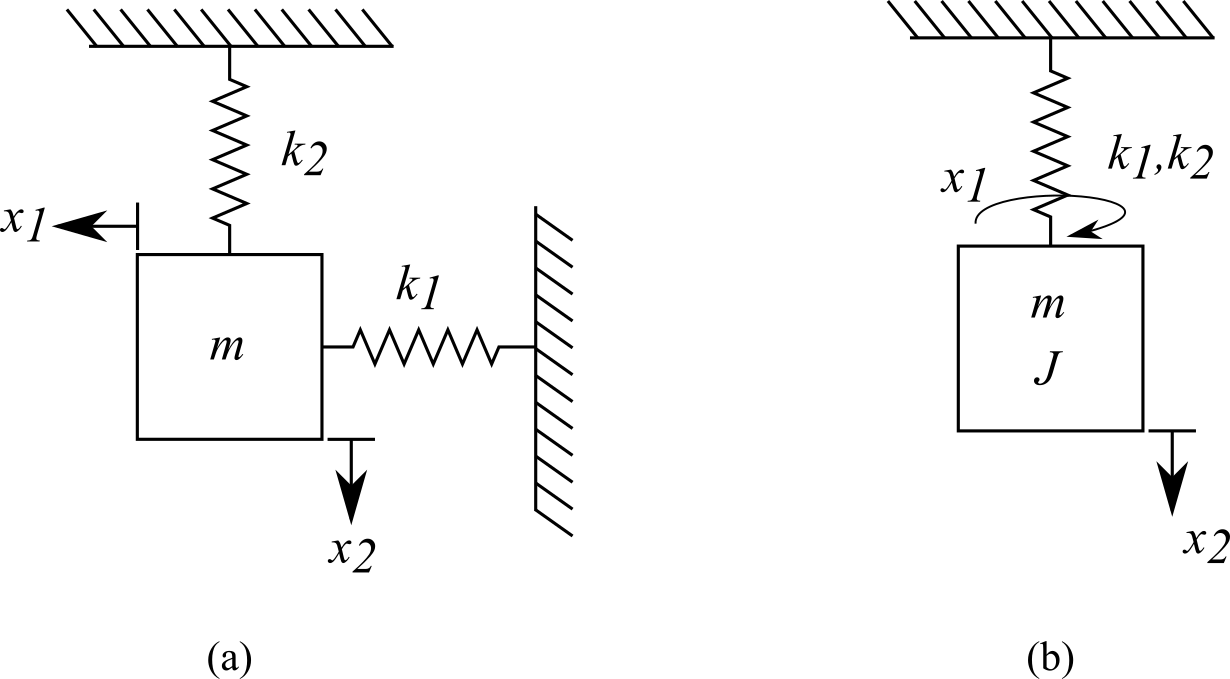
\includegraphics[]{../Figures/2-DOF-spring_mass_examples.png}
	\caption{Examples of single mass 2-DOF systems that: (a) displace in the vertical and horizontal directions; and (b) rotates about the spring and displaces in the vertical direction. }
	\label{fig:2-DOF-spring_mass_examples}
\end{figure}
Another example of a 2-DOF system with two masses, each with their own independent coordinate system, is presented in figure \ref{fig:2-DOF-spring_mass_horizontal}. The two coordinates that describe the systems movements are $x_1$ and $x_2$.
\begin{figure}[H]
	\centering
	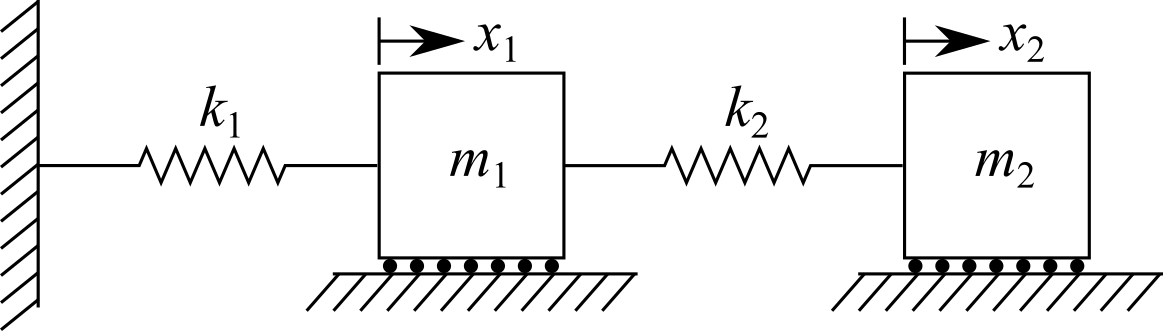
\includegraphics[]{../Figures/2-DOF-spring_mass_horizontal.png}
	\caption{2-DOF system with two masses and two independent confidante systems $x_1$ and $x_2$.}
	\label{fig:2-DOF-spring_mass_horizontal}
\end{figure}

\subsubsection{Solution for the Two-Degree-of-Freedom System}
Before we derive a model for undamped 2-DOF systems, let us first consider the solution to the system shown in figure \ref{fig:2-DOF-spring_mass_horizontal}. The solution consists of two equations, one for each mass. This solution will be derived in section \ref{sec:2-DOF_derive_solution} and is expressed by the coupled equations:
\begin{equation}
	x_1(t) = A_1 \sin (\omega_1 t + \phi_1 )u_{11}+ A_2 \sin (\omega_2 t + \phi_2 )u_{12} \hspace{3.35cm} 
\end{equation}
\begin{equation}
	x_2(t) = A_1 \sin (\omega_1 t + \phi_1 )u_{21}+ A_2 \sin (\omega_2 t + \phi_2 )u_{22} , \hspace{1cm} \omega_1 \text{ or } \omega_2 \neq 0 \nonumber
\end{equation}
These two equations ban be written as a single equation in matrix form as:
\begin{equation}
	\mathbf{x}(t) = A_1 \sin (\omega_1 t + \phi_1 )\mathbf{u}_1 + A_2 \sin (\omega_2 t + \phi_2 )\mathbf{u}_2 , \hspace{1cm} \omega_1 \text{ or } \omega_2 \neq 0
	\label{eq:2-DOF_solution}
\end{equation}
Where the bold text denotes vectors. Therefore, the vectors $\mathbf{u}_1$ and $\mathbf{u}_2$ are the mathematical expressions that ``couple'' or tie the equations together. Expanding these vectors shows: 
\begin{eqnarray}
 \mathbf{x}(t)=  \begin{bmatrix} x_1(t) \\  x_2(t) \end{bmatrix}, \hspace{2ex} \mathbf{u}_1=  \begin{bmatrix} u_{11} \\  u_{21} \end{bmatrix}, \hspace{2ex} \mathbf{u}_2=  \begin{bmatrix} u_{12} \\  u_{22} \end{bmatrix}\text{, }
\end{eqnarray}
The four key components of the solution expressed in equation \ref{eq:2-DOF_solution} are:
\begin{enumerate}
\item $\omega_1$ and $\omega_2$ are the natural frequencies of the system. They are not the frequencies of the masses. The solution states that each of the masses oscillates at the two frequencies $\omega_1$ and $\omega_2$. Moreover, consider the special case where the initial conditions are selected to force $A_2 = 0$, in this case, each mas would only oscillates at only one frequency, $\omega_1$.
\item $A_1$ and $A_2$ are the constants of integration and determine the amplitude of the system.
\item $\phi_1$ and $\phi_2$ represent the phase shift of the system
\item $\mathbf{u}_1$ and $\mathbf{u}_2$ are the first and second mode shapes of the system and couple the system together.
\end{enumerate}

\subsubsection{Deriving the Solution for the Two-Degree-of-Freedom System}
\label{sec:2-DOF_derive_solution}
To derive this solution for the system under consideration a FBD for figure \ref{fig:2-DOF-spring_mass_horizontal} can be constructed for the forces acting on each mass. First we have to make the assumption that $x_1 < x_2$, this allows us to say that $m_2$ pulls on $m_1$ and results in:
\begin{figure}[H]
	\centering
	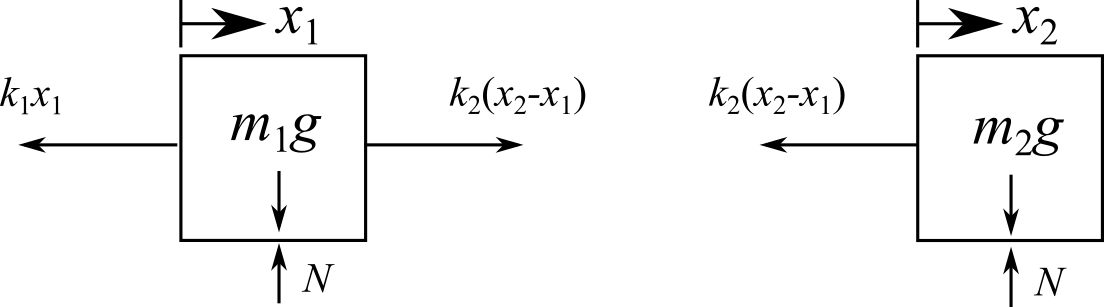
\includegraphics[]{../Figures/2-DOF-spring_mass_horizontal_FBD.png}
	\caption{Free body diagram for the 2-DOM system presented in figure \ref{fig:2-DOF-spring_mass_horizontal}.}
	\label{fig:2-DOF-spring_mass_horizontal_FBD}
\end{figure}
\noindent Applying Newton's second law and summing the forces on each mass in the horizontal direction yields:
\begin{eqnarray}
m_1\ddot{x}_1 &= & -k_1x_1 + k_2(x_2-x_1) \\
m_2\ddot{x}_2&= & -k_2(x_2-x_1)  \nonumber
\end{eqnarray}
These equations can be rearranged in terms of  $x_1$ and $x_2$ as:
\begin{eqnarray}
m_1\ddot{x}_1 +(k_1+k_2)x_1 -k_2x_2 =0 \\
m_2\ddot{x}_2 - k_2x_1 + k_2x_2 = 0 \nonumber
\end{eqnarray}
where these are two coupled second-order differential equations that each require two initial conditions to solve. These initial conditions can be obtained form the displacement and velocity terms as:
\begin{eqnarray}
x_1(0) = x_{10} \\
\dot{x}_1(0) = \dot{x}_{10} = v_{10} \nonumber \\ 
x_2(0) = x_{20} \nonumber \\ 
\dot{x}_2(0) = \dot{x}_{20} = v_{20} \nonumber
\end{eqnarray}
As before, these initial conditions will be the constants of integration used to solve the two second-order differential equations. This solution will provide the free response of each mass in the system. There is a multitude of ways to solve these two coupled  second-order differential equations, however, here we will just consider a matrix notation solution. This matrix notation solution is used as this formulation is readably solved using computers and is expandable to more than 2 DOF.

To initiate the solution, let us first develop the matrix formulation of the two coupled ODEs:
\begin{eqnarray}
  \begin{bmatrix} m_1 & 0  \\  0 & m_2 \end{bmatrix}\begin{bmatrix} \ddot{x_1} \\  \ddot{x_2} \end{bmatrix} + \begin{bmatrix} k_1+k_2 & -k_2  \\  -k_2 & k_2 \end{bmatrix}\begin{bmatrix} x_1 \\  x_2 \end{bmatrix} = \begin{bmatrix} 0 \\  0 \end{bmatrix}
\end{eqnarray}
This equation can also be expressed as the vector equation:
\begin{equation}
M\mathbf{\ddot{x}} + K\mathbf{x} =0
\end{equation}
and is known as the EOM in vector form. In this formulation the mass matrix ($M$) is defined as:
\begin{eqnarray}
 M=  \begin{bmatrix} m_1 & 0  \\  0 & m_2 \end{bmatrix}  
\end{eqnarray}
while the stiffness matrix ($K$) is:
\begin{eqnarray}
 K=  \begin{bmatrix} k_1+k_2 & -k_2  \\  -k_2 & k_2 \end{bmatrix}
\end{eqnarray}
along with the displacement, velocity, and acceleration matrices:
\begin{eqnarray}
 \mathbf{x}=  \begin{bmatrix} x_1 \\  x_2 \end{bmatrix} , \hspace{2ex} \mathbf{\dot{x}}=  \begin{bmatrix} \dot{x}_1 \\  \dot{x}_2 \end{bmatrix}, \hspace{2ex} \mathbf{\ddot{x}}=  \begin{bmatrix} \ddot{x}_1 \\  \ddot{x}_2 \end{bmatrix}
\end{eqnarray}
Beyond these equations we can write the initial conditions as:
\begin{eqnarray}
\mathbf{x_0}=  \begin{bmatrix} x_1(0) \\  x_2(0) \end{bmatrix},  \hspace{1cm} \mathbf{\dot{x}_0}=  \begin{bmatrix} \dot{x}_1(0) \\  \dot{x}_2(0) \end{bmatrix}
\end{eqnarray}
This simple connection between vibration analysis and matrix analysis allows computers to be used to solve large and complicated vibration problems quickly.

Recall that the 1-DOF version of the equation of motion was solved by calculating the values of the constants in an assumed harmonic solution. The same approach is applied here in order to solve for the displacement of the two-DOF system. This time, the the solution is assumed in the form:

\begin{equation}
	\mathbf{x}(t) = \mathbf{u}e^{j\omega t}
\end{equation}
where $\mathbf{u}$ is a vector of constants to be demerited and can be written as:
\begin{eqnarray}
\mathbf{u}=  \begin{bmatrix} u_1 \\  u_2 \end{bmatrix}
\end{eqnarray}
From before, $\omega$ is also a constant to be determined. Again, $j=\sqrt{-1}$. In the same manner as before, $e^{j\omega t}$ represents harmonic motion as $e^{j\omega t} = \cos(\omega t) + j \sin(\omega t)$. Taking the derivatives of $\mathbf{x}(t) = \mathbf{u}e^{j\omega t}$ yields:
\begin{equation}
	\dot{\mathbf{x}}(t) = j\omega\mathbf{u}e^{j\omega t}
\end{equation}
\begin{equation}
	\ddot{\mathbf{x}}(t) = -\omega^2\mathbf{u}e^{j\omega t}
\end{equation}
Substituting this into the EOM in vector form ($M\mathbf{\ddot{x}} + K\mathbf{x} =0$) yields:
\begin{equation}
-\omega^2 M  \mathbf{u}e^{j\omega t} + K\mathbf{u}e^{j\omega t} =0
\end{equation}
or 
\begin{equation}
(-\omega^2 M  + K)\mathbf{u}e^{j\omega t} =0
\end{equation}
As $e^{j\omega t} \neq 0$ for any value of $t$ and not allowing $\mathbf{u}$ to be zero it can be demerited that $(-\omega^2 M  + K)$ must satisfy the vector equation. Therefore,
\begin{equation}
(-\omega^2 M  + K)\mathbf{u} =0, \hspace{1cm} \mathbf{u}\neq0
\end{equation}
This forms a homogeneous set of algebraic equations. To be useful, these equations have a nonzero solution for the system must exist. For this to be true, the the inverse of the coefficient matrix $(-\omega^2 M  + K)$ must not exist. To expand, assume that the the inverse of $(-\omega^2 M  + K)$ does exist, by multiplying both sides of the equation by $(-\omega^2 M  + K)^{-1}$ yields $\mathbf{u}=0$. This is trivial solution (its not useful) as it no motion in the system is implied. Therefore, the logical connection can be drawn between the  solution of equation and the inverse of the coefficient matrix $(-\omega^2 M  + K)$.

Applying the singularity condition to the coefficient matrix of equation $(-\omega^2 M  + K)\mathbf{u} =0, \hspace{1ex} \mathbf{u}\neq0$ results a nonzero solution of $\mathbf{u}$. However, for this to exist the following must be true:
\begin{equation}
\det(-\omega^2 M  + K) = 0
\end{equation}
Solving this expression results in one algebraic equation with one unknown ($\omega$). Expanding the above equation to consider the values for the matrices $M$ and $K$ results in:
\begin{eqnarray}
\det\begin{bmatrix} -\omega^2 m_1 + k_1 + k_2 & -k_2  \\  -k_2 & -\omega^2 m_2 + k_2 \end{bmatrix}=0
\end{eqnarray}
Using the definition of the determinant yields that the unknown quantity $\omega^2$ must satisfy:
\begin{equation}
m_1 m_2 \omega^4 - (m_1 k_2 + m_2 k_1 + m_2 k_2)\omega^2 + k_1 k_2 = 0
\end{equation}
This expression is called the characteristic equation for the system and is used to determine the constants $\omega_{1,2}$, in the assumed form of the solution given by the assumed solution $\mathbf{x}(t) = \mathbf{u}e^{j\omega t}$, once the values of the physical parameters $m_1$, $m_2$, $k_1$, and $k_2$ are known. Note that $\omega_{1,2}$ are not in the characteristic equation, therefore, solving for $\omega_{1,2}$  will be done by factoring the equation above to obtain two solutions $\omega_1$ and $\omega_2$. The characteristic equation is in the form of the quadratic formula if you set $x=\omega^2$, as:
\begin{equation}
ax^2 + bx +c = 0
\end{equation}

After finding the value of $\omega_{1,2}$ using the characteristic equation, the values in $\mathbf{u}$ can be found using equation $(-\omega^2 M  + K)\mathbf{u} =0, \hspace{1ex} \mathbf{u}\neq0$ for each value of $\omega^2$. That is, for both $\omega_1$ and $\omega_2$ there is a vector  $\mathbf{u}$ that satisfies the equation. These solutions can be written as:
\begin{equation}
	(-\omega_1^2 M  + K)\mathbf{u}_1 =0
\end{equation}
and 
\begin{equation}
	(-\omega_2^2 M  + K)\mathbf{u}_2 =0
\end{equation}
The direction of the vectors $\mathbf{u}_1$ and $\mathbf{u}_2$ can be obtained by solving the above expressions, however, the information regarding the magnitude of is not contained in this expression. To verify this, assume that $\mathbf{u}_1$ satisfies the equation, therefore, the vector $a\mathbf{u}_1$ also satisfies the equation where $a$ is any nonzero number. Hence the vectors satisfying the above are of arbitrary magnitude.
 
The values obtained for $\mathbf{u}_1$ and $\mathbf{u}_2$ can now be combined with the assumed solution:
\begin{equation}
	\mathbf{x}(t) = \mathbf{u}e^{j\omega t}
\end{equation}
to form a set of solution:
\begin{equation}
	\mathbf{x}(t) = \mathbf{u}_1e^{-j\omega_1 t}, \hspace{2ex} \mathbf{u}_1e^{j\omega_1 t}, \hspace{2ex} \mathbf{u}_2e^{-j\omega_2 t}, \hspace{2ex} \mathbf{u}_2e^{j\omega_2 t}
\end{equation}
Since the equation to be solved is linear, the solution is the sum of these solutions. This results in:
\begin{equation}
	\mathbf{x}(t) = (a e^{j\omega_1 t} + b e^{-j\omega_1 t})\mathbf{u}_1 +(c e^{j\omega_2 t} + d e^{-j\omega_2 t})\mathbf{u}_2
\end{equation}
where $a$, $b$, $c$, and $d$ are the arbitrary constants of integration to be determined by the initial conditions. Applying Euler's formulas for the sin functions (where $\omega_1 \text{ or } \omega_2 \neq 0$) reorganizes this equation as:
\begin{equation}
	\mathbf{x}(t) = A_1 \sin (\omega_1 t + \phi_1 )\mathbf{u}_1 + A_2 \sin (\omega_2 t + \phi_2 )\mathbf{u}_2 , \hspace{1cm} \omega_1 \text{ or } \omega_2 \neq 0
\end{equation}
Another way to write this equation is in the form:
\begin{equation}
	 \begin{bmatrix} x_1(t) \\  x_2(t) \end{bmatrix} =  \begin{bmatrix} \mathbf{u}_1 & \mathbf{u}_2 \end{bmatrix}
	 \begin{bmatrix} A_1 \sin (\omega_1 t + \phi_1 )\\ A_2 \sin (\omega_2 t + \phi_2 )\end{bmatrix}, \hspace{1cm} \omega_1 \text{ or } \omega_2 \neq 0
\end{equation}
Where the values for $A_1$ and $A_2$ can be obtained by setting applying the boundary conditions and taking the derivatives of the equations as done in the 1-DOF problems. 

The final form of the equation provides a physical insight into the solution of the system. It states that the each mass in the system oscillates at both of the natural frequencies of the system ($\omega_1$ and $\omega_2$). Furthermore, the importance of the  initial conditions can be understood. Assume that initial conditions are chosen that result in $A_2=0$, this cancels out the second natural frequency such that each mass oscillates at only one frequency,  $\omega_1$. Moreover, the positions of the masses can determined by the values of the vector $\mathbf{u}_1$ at any given time. For this reason,  $\mathbf{u}_1$ is termed the first mode shape of the system. Likewise, if the opposite initial conditions are chosen such that  $A_1=0$, then both system coordinates (e.g., masses in the systems we have studied) will oscillate at $\omega_2$ and again, the positions can be obtained from the vector $\mathbf{u}_2$. Where $\mathbf{u}_2$ is termed the second mode shape. The interactions between mode shapes and natural frequencies are very important and form the basis of several area in the field of vibrations.

\begin{example}
\label{ex:2-DOF}
Considering the following system:
\begin{figure}[H]
	\centering
	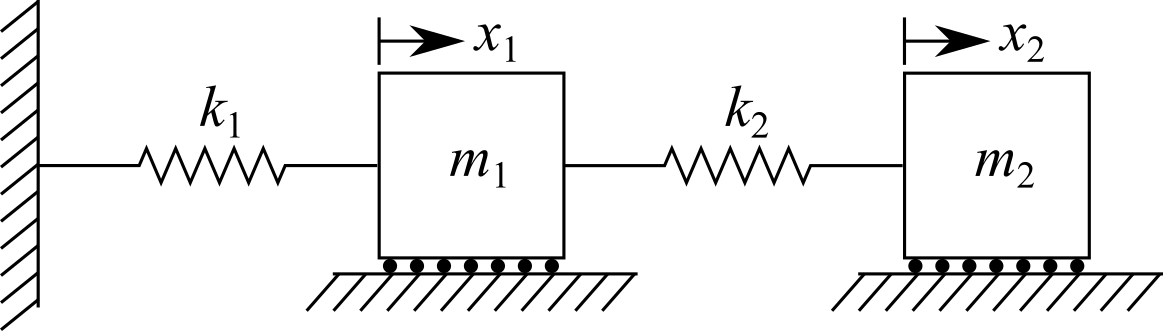
\includegraphics[]{../Figures/2-DOF-spring_mass_horizontal.png}
	\caption{2-DOF system with two masses and two independent confidante systems $x_1$ and $x_2$.}
\end{figure}
Calculate response for the system if $m_1$=9 kg, $m_2$=1 kg, $k_1$ = 24 N/m, and $k_2$ = 3 N/m with the initial conditions $x_{10}=1$ mm, $v_{10}=0$ mm/s, $x_{20}=0$ mm, and $v_{20}=0$ mm/s. \\


\textbf{Solution:} We have already obtained a characteristic equation for this system, given as:
\begin{equation}
m_1 m_2 \omega^4 - (m_1 k_2 + m_2 k_1 + m_2 k_2)\omega^2 + k_1 k_2 = 0
\end{equation}
Substituting our values into this obtains:
\begin{equation}
9 \cdot 1 \omega^4 - (9 \cdot 3 + 1 \cdot 24 + 1 \cdot 3)\omega^2 + 24 \cdot 3 = 0
\end{equation}
or
\begin{equation}
\omega^4 - 6\omega^2 + 8 =0
\end{equation}
This can then be factored into:
\begin{equation}
(\omega^2-2)(\omega^2-4)=0
\end{equation}
This results in solutions of $\omega^2_1 = 2$ and $\omega^2_2 = 4$. Leading to:
\begin{equation}
\omega_1 = \pm \sqrt{2} \text{ rad/sec}, \hspace{2ex} \omega_2 = \pm 2 \text{ rad/sec}
\end{equation}
Next, we need to obtain solutions for $\mathbf{u}_1$ and $\mathbf{u}_2$. Having solved for $\omega_1$ and $\omega_2$ we can obtained. First, knowing $\mathbf{u}_1 = [u_{11} u_{21}]^\text{T}$ and using $\omega_1 = \sqrt{2}$ and the follwoing equation:
\begin{equation}
	(-\omega_1^2 M  + K)\mathbf{u}_1 =0
\end{equation}
yields
simplified to
\begin{equation}
	 \bigg(-2\begin{bmatrix} 9 & 0 \\   0  & 1 \end{bmatrix} + \begin{bmatrix} 24+3 & -3 \\    -3  & 3 \end{bmatrix}\bigg)\begin{bmatrix} u_{11}\\ u_{21}\end{bmatrix} = \begin{bmatrix} 0\\ 0\end{bmatrix}
\end{equation}
simplified to
\begin{equation}
	 \begin{bmatrix} 27-9\cdot 2 & -3 \\    -3  & 3-2 \end{bmatrix} 
	 \begin{bmatrix} u_{11}\\ u_{21}\end{bmatrix}=\begin{bmatrix} 0\\ 0\end{bmatrix}
\end{equation}
or
\begin{equation}
	 \begin{bmatrix} 9 & -3 \\    -3  & 1 \end{bmatrix} 
	 \begin{bmatrix} u_{11}\\ u_{21}\end{bmatrix}=\begin{bmatrix} 0\\ 0\end{bmatrix}
\end{equation}
Taking the dot product of the matrix equation yields:
\begin{equation}
	9u_{11} -3u_{21}=0 \text{, and } -3u_{11} + u_{21}=0
\end{equation}
Both of these equations yield the same equation, that is:
\begin{equation}
	\frac{u_{11}}{u_{21}} =\frac{1}{3}
\end{equation}
As mentioned before, only the ratio of the elements is determined here. To show this is true it is easily seen that:
\begin{equation}
	u_{11}=u_{21}\frac{1}{3} \rightarrow  a u_{11}= a u_{21}\frac{1}{3} 
\end{equation}
To obtain a numerical value, we arbitrarily assign a value to one of the elements. Here, let $u_{21}=1$ so  let $u_{11}=1/3$. Therefore, 
\begin{equation}
	 \textbf{u}_1 = \begin{bmatrix} \frac{1}{3}\\ 1\end{bmatrix}
\end{equation}
The same processes can be used for obtaining $\textbf{u}_1$ using $\omega_2=2$, this results in:
\begin{equation}
	 \begin{bmatrix} -9 & -3 \\    -3  & -1 \end{bmatrix} 
	 \begin{bmatrix} u_{12}\\ u_{22}\end{bmatrix}=\begin{bmatrix} 0\\ 0\end{bmatrix}
\end{equation}
Taking the dot product of the matrix equation yields:
\begin{equation}
	-9u_{12} -3u_{22}=0 \text{, and } -3u_{12} - u_{22}=0
\end{equation}
Both of these equations yield the same equation, that is:
\begin{equation}
	\frac{u_{12}}{u_{22}} =-\frac{1}{3}
\end{equation}
Again, assuming $u_{22}=1$  this can be rearranged into $\textbf{u}_2$ as:
\begin{equation}
	 \textbf{u}_2 = \begin{bmatrix} -\frac{1}{3}\\ 1\end{bmatrix}
\end{equation}
Where $\mathbf{u}_1$ and $\mathbf{u}_2$ represent only the directions and shape of the mode shapes and not the magnitude of the mode shapes. 
Now that we have the mode shapes, we can solve for the initial conditions $A_1$ and $A_2$. To do this, let us use the following formulation of the solution:
\begin{equation}
	 \begin{bmatrix} x_1(t) \\  x_2(t) \end{bmatrix} =  \begin{bmatrix} \mathbf{u}_1 & \mathbf{u}_2 \end{bmatrix}
	 \begin{bmatrix} A_1 \sin (\omega_1 t + \phi_1 )\\ A_2 \sin (\omega_2 t + \phi_2 )\end{bmatrix}, \hspace{1cm} \omega_1 \text{ or } \omega_2 \neq 0
\end{equation}
Adding our values for the problem at $t=0$ this becomes:
\begin{equation}
	 \begin{bmatrix} 1 \\  0 \end{bmatrix} =  \begin{bmatrix} \frac{1}{3} & -\frac{1}{3} \\ 1 & 1 \end{bmatrix}
	 \begin{bmatrix} A_1 \sin (\sqrt{2} t + \phi_1 )\\ A_2 \sin (2 t + \phi_2 )\end{bmatrix}
\end{equation}
and after applying the dot product:
\begin{equation}
	 \begin{bmatrix} 1 \\  0 \end{bmatrix} =  \begin{bmatrix} \frac{1}{3}A_1 \sin (\phi_1 ) -\frac{1}{3}A_2 \sin (\phi_2)\\ A_1 \sin (\phi_1 )+A_2 \sin (\phi_2 )\end{bmatrix}
\end{equation}
Next we can differentiate the equation for $x(t)$ to obtain the velocity solution. Adding our values for the problem at $t=0$ obtains:
\begin{equation}
	 \begin{bmatrix} \dot{x}_1(0) \\  \dot{x}_2(0) \end{bmatrix}  = \begin{bmatrix} v_{10} \\  v_{20} \end{bmatrix} = \begin{bmatrix} 0 \\  0 \end{bmatrix} =   \begin{bmatrix} \frac{\sqrt{2}}{3}A_1 \cos (\phi_1 ) -\frac{2}{3}A_2 \cos (\phi_2)\\ \sqrt{2}A_1 \cos (\phi_1 )+2 A_2 \cos (\phi_2 )\end{bmatrix}
\end{equation}
Now that we have 4 equations for 4 unknowns we can use these equations to solve for $A_1$,  $A_2$, $\phi_1$,  and $\phi_2$. The 4 equations are:
\begin{equation}
3= A_1 \sin (\phi_1 ) - A_2 \sin (\phi_2)
\end{equation}
\begin{equation}
0= A_1 \sin (\phi_1 ) + A_2 \sin (\phi_2)
\end{equation}
\begin{equation}
0= \sqrt{2}A_1 \cos (\phi_1 ) - 2A_2 \cos (\phi_2)
\end{equation}
\begin{equation}
0= \sqrt{2}A_1 \cos (\phi_1 ) + 2A_2 \cos (\phi_2)
\end{equation}
Setting these last two equations equal to each other yields:
\begin{equation}
0= \sqrt{2}A_1 \cos (\phi_1 ) + 2A_2 \cos (\phi_2) = \sqrt{2}A_1 \cos (\phi_1 ) - 2A_2 \cos (\phi_2)
\end{equation}
or:
\begin{equation}
0= - 4A_2 \cos (\phi_2)
\end{equation}
For this equation to be true, $\phi_2=\frac{\pi}{2}$. Therefore, applying this to $0= \sqrt{2}A_1 \cos (\phi_1 ) + 2A_2 \cos (\phi_2)$ results in:
\begin{equation}
0= \sqrt{2}A_1 \cos (\phi_1 )
\end{equation}
where again, for this equation to be true, $\phi_1=\frac{\pi}{2}$. Now the first two equations become:
\begin{equation}
3= A_1 - A_2 
\end{equation}
\begin{equation}
0= A_1 + A_2 
\end{equation}
Where this shows us that $A_1 = \frac{3}{2}$ mm and $A_2 = -\frac{3}{2}$. Therefore, now that we have the initial conditions we can find a solution for the temporal response of each mass. Using the equations from before:
\begin{equation}
	x_1(t) = A_1 \sin (\omega_1 t + \phi_1 )u_{11} + A_2 \sin (\omega_2 t + \phi_2 )u_{12}
\end{equation}
\begin{equation}
	x_2(t) = A_1 \sin (\omega_1 t + \phi_1 )u_{21} + A_2 \sin (\omega_2 t + \phi_2 )u_{22}
\end{equation}
And applying our obtained values
\begin{equation}
	x_1(t) = \frac{3}{2} \sin (\sqrt{2} t + \frac{\pi}{2} )\frac{1}{3} + \bigg(-\frac{3}{2}\bigg) \sin (2 t + \frac{\pi}{2} ) \bigg(-\frac{1}{3}\bigg)
\end{equation}
\begin{equation}
	x_2(t) = \frac{3}{2} \sin (\sqrt{2} t + \frac{\pi}{2} ) + \bigg(-\frac{3}{2}\bigg) \sin (2 t + \frac{\pi}{2} )
\end{equation}
results in:
\begin{equation}
	x_1(t) = \frac{1}{2} \bigg(  \sin (\sqrt{2} t + \frac{\pi}{2} ) + \sin (2 t + \frac{\pi}{2} ) \bigg)
\end{equation}
\begin{equation}
	x_2(t) = \frac{3}{2}  \bigg( \sin (\sqrt{2} t + \frac{\pi}{2} ) -\sin (2 t + \frac{\pi}{2} ) \bigg)
\end{equation}
These results can be plotted as:
\begin{figure}[H]
	\centering
	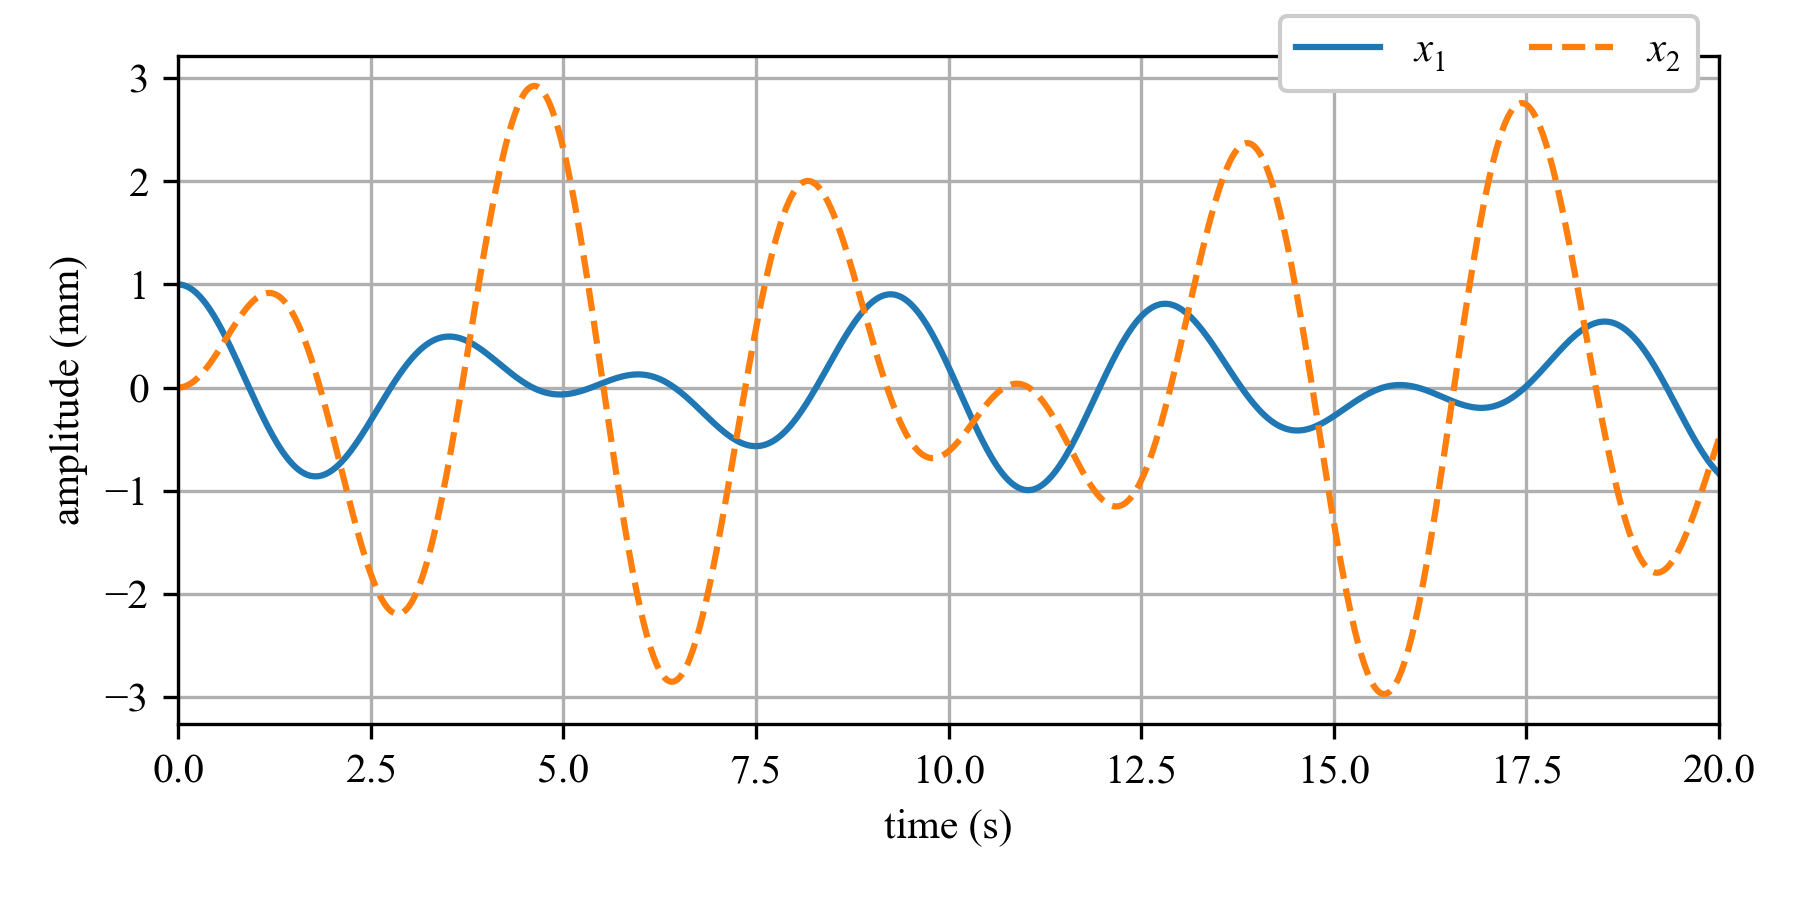
\includegraphics[width=0.9\textwidth]{../Figures/2-DOF_response.png}
	\caption{Temporal response for each of the rigid bodies in the 2-DOF system.}
\end{figure}
\end{example}


\subsubsection{Mode Shapes}
\label{sec:Mode_Shapes}

Studying and characterizing the natural frequencies of a system allows for the detailed investigation of the system response. Modern vibration analysis relies heavily on the concepts of mode shapes for various engineering tasks. Mode shapes can be better understood through a graphical representation. To do this, consider the 2-DOF system presented in figure \ref{fig:2-DOF-spring_mass_vertical}(a). Assuming that $x_1<x_2$ the FBD for the system is expressed in figure figure \ref{fig:2-DOF-spring_mass_vertical}(b).

\begin{figure}[H]
	\centering
	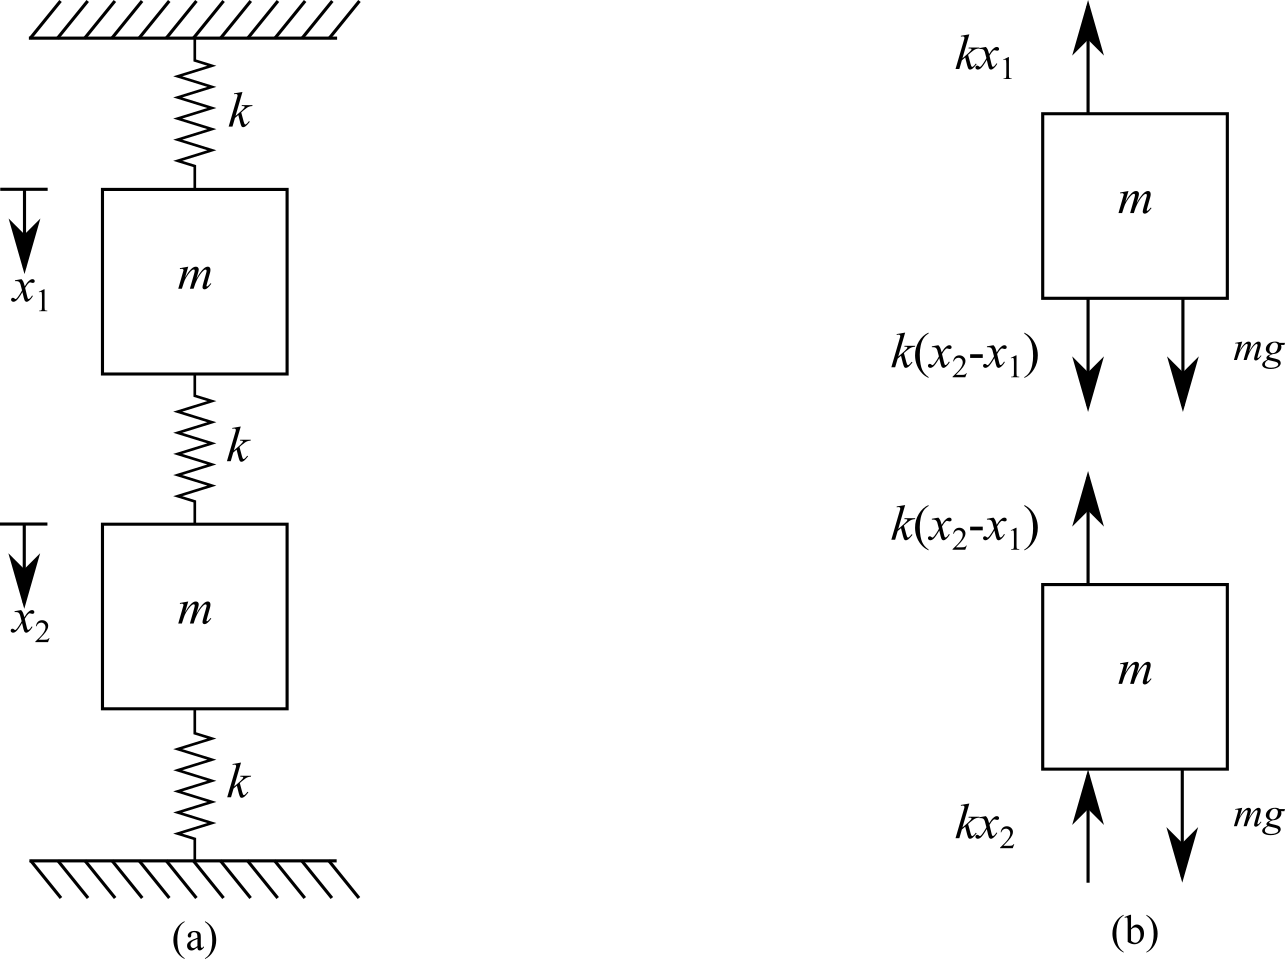
\includegraphics[]{../Figures/2-DOF-spring_mass_vertical_with_FBD.png}
	\caption{(a) 2-DOF system with two masses arranged in a vertical configuration; and (b) FBD of system.}
	\label{fig:2-DOF-spring_mass_vertical}
\end{figure}
\noindent For simplicity, all masses and spring stiffness are considered equal and that $m=1$ and $k=1$. From the previous investigations in this text we know that the forces caused by gravity will cancel out. Therefore, the EOM for the system can be written as:
\begin{eqnarray}
m_1\ddot{x}_1 &= & -kx_1 + k(x_2-x_1) \\
m_2\ddot{x}_2&= & -k(x_2-x_1) -kx_2 \nonumber
\end{eqnarray}
These equations can be written in matrix notation as:
\begin{eqnarray}
	\begin{bmatrix} m & 0  \\  0 & m \end{bmatrix}\begin{bmatrix} \ddot{x_1} \\  \ddot{x_2} \end{bmatrix} + \begin{bmatrix} 2k & -k  \\  -k & 2k \end{bmatrix}\begin{bmatrix} x_1 \\  x_2 \end{bmatrix} = \begin{bmatrix} 0 \\  0 \end{bmatrix}
\end{eqnarray}
Substituting the values of the matrices $M$ and $K$ into this expression $\det(-\omega^2 M  + K) = 0$ yields: 
\begin{eqnarray}
\det\begin{bmatrix} -\omega^2 m + 2k & -k  \\  -k & -\omega^2 m + 2k \end{bmatrix}=0
\end{eqnarray}
The determinant yields that the unknown quantity, $\omega^2$, must satisfy:
\begin{equation}
m^2 \omega^4 - 4km\omega^2 + 3k = 0
\end{equation}
Therefore, 
\begin{equation}
\omega_1 \pm \sqrt{\frac{k}{m}}=1 \text{ rad/sec}, \hspace{2ex} \omega_2 \pm \sqrt{\frac{3k}{m}}=\sqrt{3} \text{ rad/sec}
\end{equation}
Now, we need to obtain solutions for $\mathbf{u}_1$ and $\mathbf{u}_2$. Knowing $(-\omega_1^2 M  + K)\mathbf{u}_1 =0$ yields:
\begin{equation}
	 \begin{bmatrix} 1 & -1 \\    -1  & 1 \end{bmatrix} 
	 \begin{bmatrix} u_{11}\\ u_{21}\end{bmatrix}=\begin{bmatrix} 0\\ 0\end{bmatrix}
\end{equation}
Taking the dot product of the matrix equation yields:
\begin{equation}
	u_{11} - u_{21}=0 \text{, and } - u_{11} + u_{21}=0
\end{equation}
Setting $u_{11} = 1$ results in $u_{21} = 1$ . The same processes can be performed for $\mathbf{u}_2$ to show that if we set $u_{12} = 1$, $u_{22} = -1$. Therefore, the mode shapes can be expresses as:
\begin{equation}
	 \begin{bmatrix} \mathbf{u}_1 & \mathbf{u}_2 \end{bmatrix} = \begin{bmatrix}  u_{11} & u_{12} \\ u_{21} & u_{22} \end{bmatrix} = \begin{bmatrix}  1 & 1 \\ 1 & -1 \end{bmatrix}
\end{equation}
The displacement of the masses as a function of time and the general mode shape plots are graphically represented in figure \ref{fig:2-DOF_mode_shape}. In the 2-DOF system considered here, the second mode shape has a spot at the center of the middle spring spring that does not move (i.e. has zero displacement). This point is called a node. Nodes correspond to points in the mode shape where the displacement is always zero. Furthermore, the displacement of the node points remain zero at all times, as diagrammed in the top-right of figure \ref{fig:2-DOF_mode_shape}.

\begin{figure}[H]
	\centering
	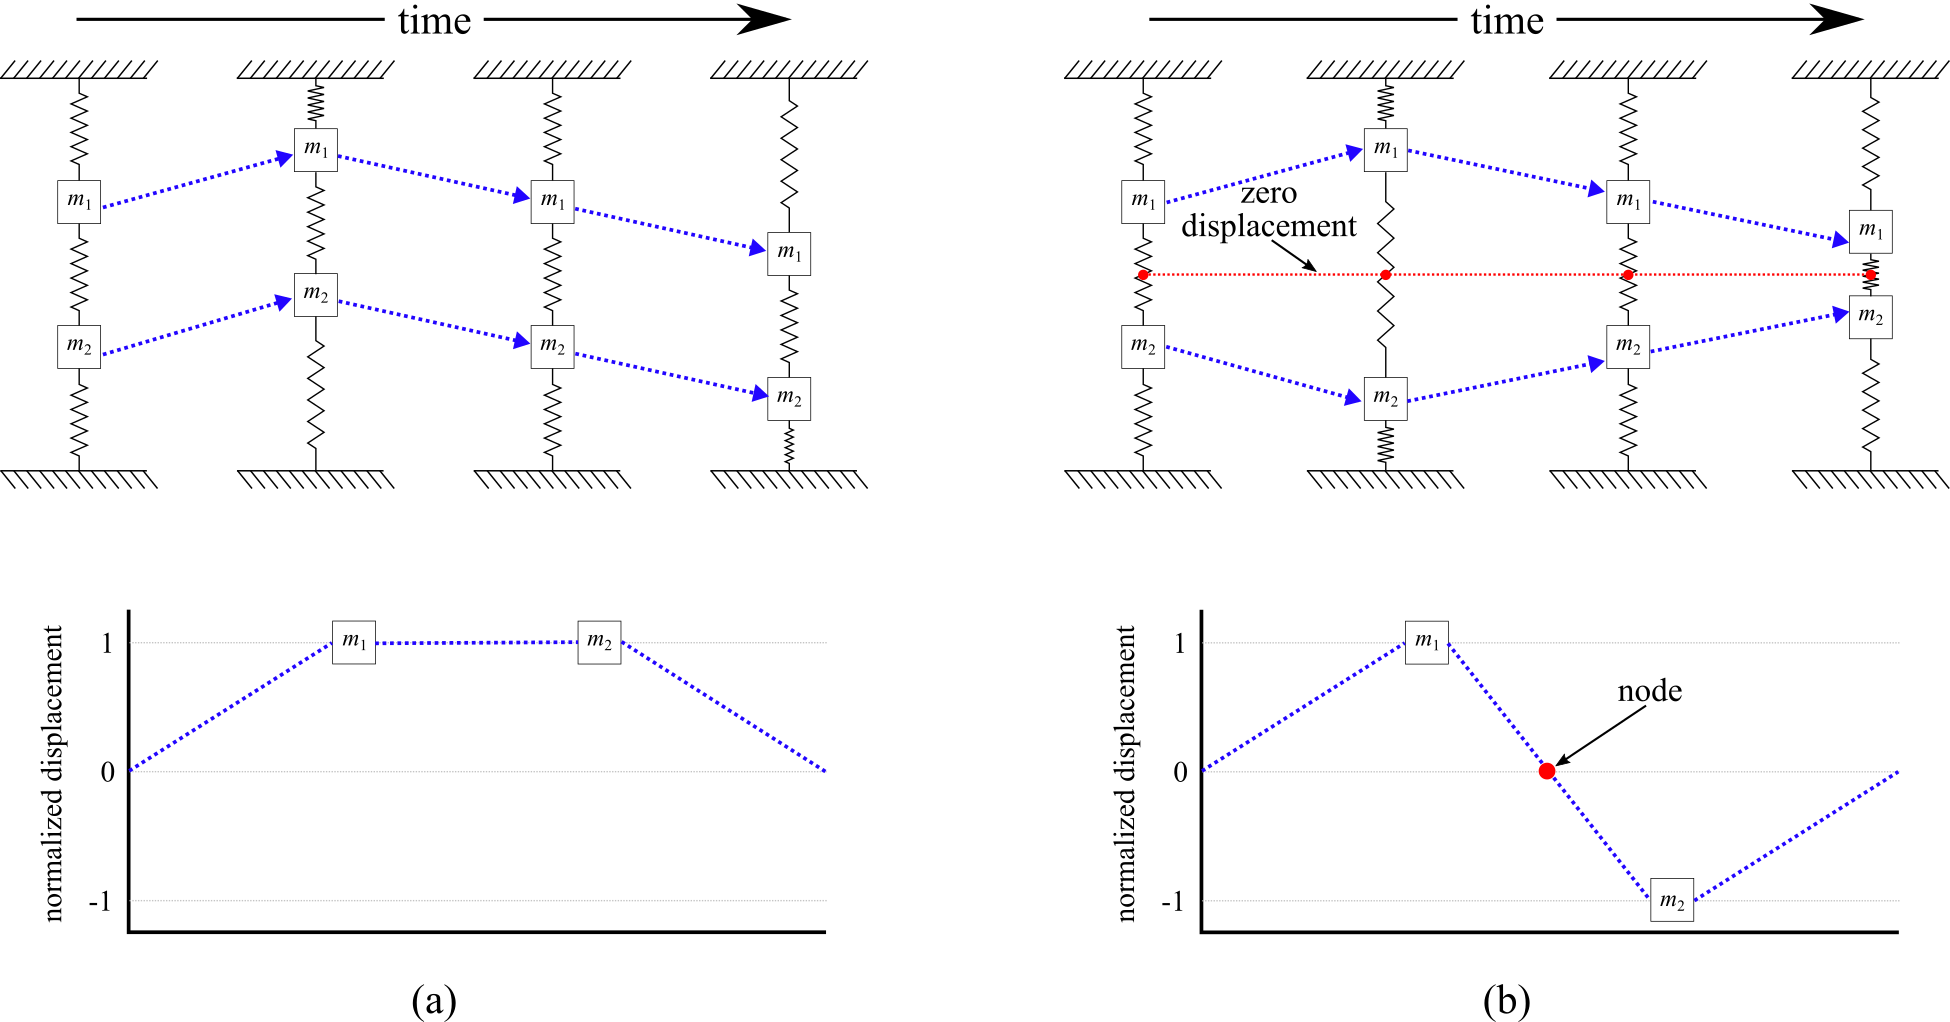
\includegraphics[]{../Figures/2-DOF_mode_shape.png}
	\caption{Modes of vibration for the system shown in figure \ref{fig:2-DOF-spring_mass_vertical} showing the: (a) first mode; and (b) second mode.}
	\label{fig:2-DOF_mode_shape}
\end{figure}


\subsection{Eigenvalue-based Solution for Natural Frequencies and Mode Shapes}

The process of calculating the mode shapes presented in sections \ref{sec:2-DOF_derive_solution} and \ref{sec:Mode_Shapes} is long and tedious. Therefore, methods that can be easily deployed on computers are of great interest to the practitioner. An eigenvalue-based solution that takes advantage of the symmetry in the $M$ and $K$ matrices and can be easily implemented on a computer is discussed in this section. 

\begin{review}

	In linear algebra, eigenvalues and eigenvectors are concepts that appear prominently in the analysis of linear transformations. By definition, If  $\textbf{v}$ is a vector (in vector space $V$ over a field $F$) and $T$ is a linear transformation into itself, then $\textbf{v}$ is an eigenvector of $T$ if $T\textbf{v}$ is a scalar multiple of $\textbf{v}$:
	\begin{equation}
	T\textbf{v} = \lambda\textbf{v}
	\end{equation}
	where $\lambda$ is a scalar in the field $F$, known as the eigenvalue associated with the eigenvector $v$.

	A matrix is positive definite if the scalar $\textbf{x}^{\text{T}}A\textbf{x}$ is positive for any non-zero vector $x$ comprised of real numbers:
	\begin{equation}
	\textbf{x}^{\text{T}}A\textbf{x} > 0
	\end{equation}
	
	The Cholesky decomposition of a real positive-definite matrix $A$ is a decomposition of the form:
	\begin{equation}
	A=LL^{\text{T}}
	\end{equation}
	where $L$ is the lower triangular matrix of $A$.

\end{review}

\subsubsection{Cholesky Decomposition}
The vast majority of mass and stiffness matrices are symmetric and positive definite due to the physical meaning of these matrices. Therefore, $M$ can be factored into two terms using the Cholesky decomposition:
\begin{equation}
	M=LL^{\text{T}}
\end{equation}
For diagonal mass matrices (all the mass values lie along the diagonal of the matrix) the Cholesky decomposition ($L$) is defined as:
\begin{equation}
	L = M^{1/2} = \begin{bmatrix} \sqrt{m_1} & 0 \\  0  & \sqrt{m_2} \end{bmatrix} 
\end{equation}
This expression factors into:
\begin{equation}
	M = M^{1/2}M^{1/2}
\end{equation}
Moreover, the inverse of the diagonal matrix ($M^{1/2}$) is denoted as $M^{-1/2}$ and defined as:
\begin{equation}
	L^{-1} = M^{-1/2} = \begin{bmatrix} \frac{1}{\sqrt{m_1}} & 0 \\  0  & \frac{1}{\sqrt{m_2}} \end{bmatrix} 
\end{equation}

\subsubsection{Deriving the Eigenvalue-based Solution}
 
To derive an eigenvalue-based solution for calculating the natural frequencies and mode shapes let us consider the previously derived EOM for a undamped 2-DOF system:
\begin{equation}
M\mathbf{\ddot{x}} + K\mathbf{x} =0
\end{equation}
This expression can be transformed into a symmetric eigenvalue problem, allowing us to leverage the strengths of symmetric eigenvalue mathematics and computer solvers. To perform this transform, we set $\mathbf{x}=M^{-1/2}\mathbf{q}$ and multiply the equation by $M^{-1/2}$ such that the EOM becomes:
\begin{equation}
M^{-1/2}MM^{-1/2}\mathbf{\ddot{q}} + M^{-1/2}KM^{-1/2}\mathbf{q} =0
\end{equation}
As $M^{-1/2}MM^{-1/2}$ is equal to the identity matrix $I$ and defining $M^{-1/2}KM^{-1/2}$ as the mass normalized stiffness $\widetilde{K}$ yields the simplified expression:
\begin{equation}
I\mathbf{\ddot{q}} + \widetilde{K}\mathbf{q} =0
\end{equation}
where $\widetilde{K}=M^{-1/2}KM^{-1/2}$ is analogous to $\sqrt{k/m}$ from the 1-DOF system. 

As before, a solution is found by assuming a solution, taking the derivatives of the solution and substituting it into the EOM. Following these steps and assuming a solution of:
\begin{equation}
\mathbf{q} = \textbf{v}e^{j\omega t}
\end{equation}
results in an EOM in the from:
\begin{equation}
-\textbf{v} \omega^2 e^{j\omega t} + \widetilde{K}\textbf{v}e^{j\omega t} =0
\end{equation}
diving out the nonzero scaler $e^{j\omega t}$ and rearranging the above expression results in:
\begin{equation}
\widetilde{K}\textbf{v} =  \omega^2 \textbf{v}
\end{equation}
Knowing that $\textbf{v}\neq0$, as a vector with zeros would mean no motion is present in the system, this equation can be expressed in a typical eigenvalue formulation:
\begin{equation}
\widetilde{K}\textbf{v} =  \lambda \textbf{v}
\label{eq:eigenvalue_problem}
\end{equation}
where $\lambda = \omega^2 $. Or more importantly, $\omega = \sqrt{\lambda}$. As $\widetilde{K}$ is symmetric, this is a symmetric eigenvalue problem. Moreover, the vector $\lambda$ represent the eigenvalues of the system. Given that  we set $\mathbf{x}=M^{-1/2}\mathbf{q}$, the eigenvectors are not a direct representation of the mode shapes. To develop a link between the eigenvectors and mode shapes we first need to normalize the lengths of the eigenvectors obtained by solving equation \ref{eq:eigenvalue_problem} to that of a unit vector. The norm of a unit vector is defined as:
\begin{equation}
1= ||\textbf{v}|| = \sqrt{\textbf{v}^{\text{T}}\textbf{v}} = \sqrt{\sum_{i=1}^{n}(v_i^2)}
\end{equation} 
where a scalar is used in conjunction with vector such that $\alpha\textbf{u}=1$ computed the normalized unit vector directions as outlined in example \ref{ex:vector_normalizeation}. In general, a nonzero vector of any length can be normalized by calculating:
\begin{equation}
\frac{1}{\sqrt{\textbf{v}^{\text{T}}\textbf{v}} } \textbf{v}
\end{equation} 


We can relate the eigenvectors to the modes shapes by a factor of the mass matrix:
\begin{equation}
\textbf{u}_1 = M^{-1/2}\textbf{v}_1
\end{equation}
The important thing to remember is that the natural frequencies are the square root of the eigenvalues and the mode shapes are related to the eigenvectors through the mass matrix. 


\begin{example}
\label{ex:vector_normalizeation}
Normalize the vector $\textbf{v}_1=[1/3 \hspace{1ex} 1]^T$

\textbf{Solution:} To normalize the vector $\textbf{v}_1$, a scalar ($\alpha$) is calculated to make $\alpha\textbf{v}=1$.  Therefore, following the definition of an orthogonal vector:
\begin{equation}
(\alpha \textbf{v}_1)^T(\alpha \textbf{v}_1) = 1
\end{equation}
or:
\begin{equation}
\alpha [1/3 \hspace{1ex} 1]\alpha  \begin{bmatrix} \frac{1}{3}\\  1 \end{bmatrix}  = \alpha^2(1/9+1) = 1
\end{equation}
Therefore, $\alpha=3/\sqrt{10}$. Resulting in a normalized unit vector of $\alpha\textbf{v}_1=[1/\sqrt{10} \hspace{1ex} 3/\sqrt{10}]^T$

\end{example}



\begin{example}
Consider the system presented in example \ref{ex:2-DOF} and repeated below where $m_1$=9 kg, $m_2$=1 kg, $k_1$ = 24 N/m, and $k_2$ = 3 N/m with the initial conditions $x_{10}=1$ mm, $v_{10}=0$ mm/s, $x_{20}=0$ mm, and $v_{20}=0$ mm/s. Calculate the natural frequencies and the mode shapes using the eigenvalue solution. 
\begin{figure}[H]
	\centering
	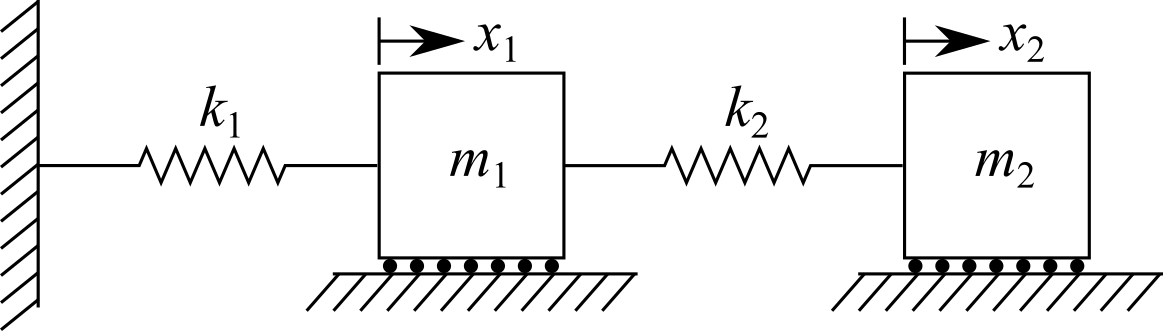
\includegraphics[]{../Figures/2-DOF-spring_mass_horizontal.png}
	\caption{2-DOF system with two masses and two independent confidante systems $x_1$ and $x_2$.}
\end{figure}




\textbf{Solution:} Writing the mass and stiffness matrix of the system as:

\begin{equation}
	M = \begin{bmatrix} 9 & 0 \\  0  & 1 \end{bmatrix} 
\end{equation}
and 
\begin{equation}
	 K = \begin{bmatrix} 27 & -3 \\    -3  & 3 \end{bmatrix}
\end{equation}
we can compute  $\widetilde{K}$ using the following expression:
\begin{equation}
	 \widetilde{K}=M^{-1/2}KM^{-1/2}
\end{equation}
where $KM^{-1/2}$ is computed first to maintain symmetry. This results in:
\begin{equation}
	 KM^{-1/2} =  \begin{bmatrix} 27 & -3 \\    -3  & 3 \end{bmatrix}  \begin{bmatrix} \frac{1}{3} & 0 \\    0  & 1 \end{bmatrix}= \begin{bmatrix} 9 & -3 \\    -1  & 3 \end{bmatrix}
\end{equation}
and:
\begin{equation}
	  \widetilde{K}=M^{-1/2}KM^{-1/2} =  \begin{bmatrix} \frac{1}{3} & 0 \\    0  & 1 \end{bmatrix} \begin{bmatrix} 9 & -3 \\    -1  & 3 \end{bmatrix}  =  \begin{bmatrix} 3 & -1\\  -1  & 3 \end{bmatrix} 
\end{equation}
Now a solution must be obtained for the eigenvalue problem:
\begin{equation}
\widetilde{K}\textbf{v} =  \lambda \textbf{v}
\end{equation}
While this can be obtained using computers for such a simple case it is more appropriate to solve this expression by had. Therefore, the above expression can be rewritten as:
\begin{equation}
(\widetilde{K} - \lambda I)\textbf{v} =  0
\end{equation}
as $\textbf{v} \neq 0$ the matrix must be singular, resulting in the determinant of the matrix equaling zero. Or:
\begin{equation}
\det \begin{bmatrix} 3-\lambda & -1 \\    -1  & 3-\lambda \end{bmatrix}  =  0
\end{equation}
This can be expanded ot the characteristic equation:
\begin{equation}
\lambda^2 -6\lambda + 8  =  0
\end{equation}
with the roots (eigenvalues):
\begin{equation}
\lambda_1 = 2\text{ and } \lambda_2 = 4
\end{equation}
Therefore, $\omega_1=\sqrt{2}$ and $\omega_2=2$. These are the same values computed in example \ref{ex:2-DOF}. The eigenvectors for $\lambda_1$ are computed as:
\begin{equation}
(\widetilde{K} - \lambda_1 I)\textbf{v} =  0
\end{equation}
or:
\begin{equation}
\begin{bmatrix} 3-2 & -1 \\    -1  & 3-2 \end{bmatrix} \begin{bmatrix} v_{11} \\ v_{21}  \end{bmatrix} =  \begin{bmatrix} 0 \\ 0  \end{bmatrix}
\end{equation}
This results in two dependent scalar equations:
\begin{equation}
v_{11} - v_{21} = 0 \text{ and } -v_{11} + v_{21} =0
\end{equation}
That show us that $v_{11} = v_{21}$ or $\textbf{v}_1=[1 \hspace{1ex} 1]^T$. Therefore, using $(\alpha \textbf{v}_1)^T(\alpha \textbf{v}_1) = 1$ we obtain:
\begin{equation}
\alpha [1 \hspace{1ex} 1]\alpha  \begin{bmatrix} 1 \\  1 \end{bmatrix}  = \alpha^2(2) = 1
\end{equation}
or $\alpha = 1/\sqrt{2}$. This allows us to normalize the vector knowing $\alpha \textbf{v}_1=1$, resulting in a normalized vector of:
\begin{equation}
\alpha \textbf{v}_1=  \frac{1}{\sqrt{2}} \begin{bmatrix} 1 \\ 1 \end{bmatrix} 
\end{equation} 
A similar processes is followed for $\lambda_2=4$ that leads to the normalized vector 
\begin{equation}
\alpha \textbf{v}_2=  \frac{1}{\sqrt{2}} \begin{bmatrix} -1 \\ 1 \end{bmatrix} 
\end{equation} 
Lastly, the normalized eigenvectors can be converted to mode shapes using $\textbf{u} = M^{-1/2}\textbf{v}$. Resulting in: 
\begin{eqnarray}
\textbf{u}_1 =  \begin{bmatrix} \frac{1}{3} & 0  \\  0 & 1 \end{bmatrix}   \begin{bmatrix} 1 \\  1 \end{bmatrix} =  \begin{bmatrix} \frac{1}{3} \\  1 \end{bmatrix}
\end{eqnarray}
and:
\begin{eqnarray}
\textbf{u}_2 =  \begin{bmatrix} \frac{1}{3} & 0  \\  0 & 1 \end{bmatrix}   \begin{bmatrix} -1 \\  1 \end{bmatrix} =  \begin{bmatrix} -\frac{1}{3} \\  1 \end{bmatrix}
\end{eqnarray}
Therefore, the first mode shape is $[1 \hspace{1ex} 1]$ while the second mode shape is $[\frac{1}{3} \hspace{1ex} -\frac{1}{3}]$. Again, this is using our prior definition of mode shapes to set $[1 \hspace{1ex} 1]$ as the first mode shape. Note that these are the same mode shape vectors as computed in example \ref{ex:2-DOF}.
\end{example}


\end{document}














